\chapter{Procedimento Experimental}\label{procedimento}

\section{Primeiro teste}\label{sec:primeiro_teste}

No primeiro teste, a mangueira utilizada para conectar a garrafa PET e o filtro
prensa, não permitia escoamento de toda a solução, por possuir em sua
extremidade um conector que obstruia a extremidade da mangueira, não permitindo
a entrada das partículas em suspensão. Foi retirado o conector, porém a conexão
entre a mangueira e a garrafa não estava totalmente vedada e não havia pressão
suficiente para que a solução entrasse na mangueira e chegasse ao filtro. Neste
teste pouca solução chegava ao filtro e saía apenas pela primeira membrana.

\begin{figure}[H]
  \centering
  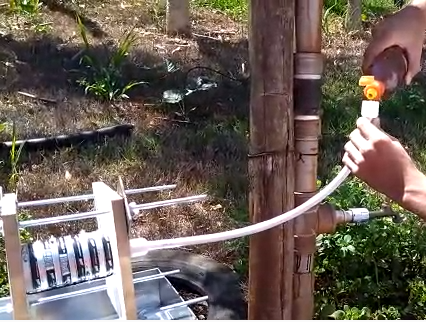
\includegraphics[width=0.9\textwidth]{figuras/primeiro_teste.png}
  \caption{Execução do primeiro teste.\label{fig:primeiro_teste}}
\end{figure}


\section{Segundo teste}\label{sec:segundo_teste}

Neste teste, utilizou-se outra garrafa, com intenção de promover mais pressão ao
sistema através da compressão da mesma. A solução foi para o filtro sem vazão
constante, sem pressão suficiente, e ainda havia vazamento na entrada do filtro.
O filtrado estava saindo em grande parte antes da primeira membrana (entre a
placa de madeira e a primeira membrana filtrante) e também antes da madeira.
Logo, a solução não estava passando nas membranas filtrantes e não estava sendo
filtrada.

\begin{figure}[H]
  \centering
  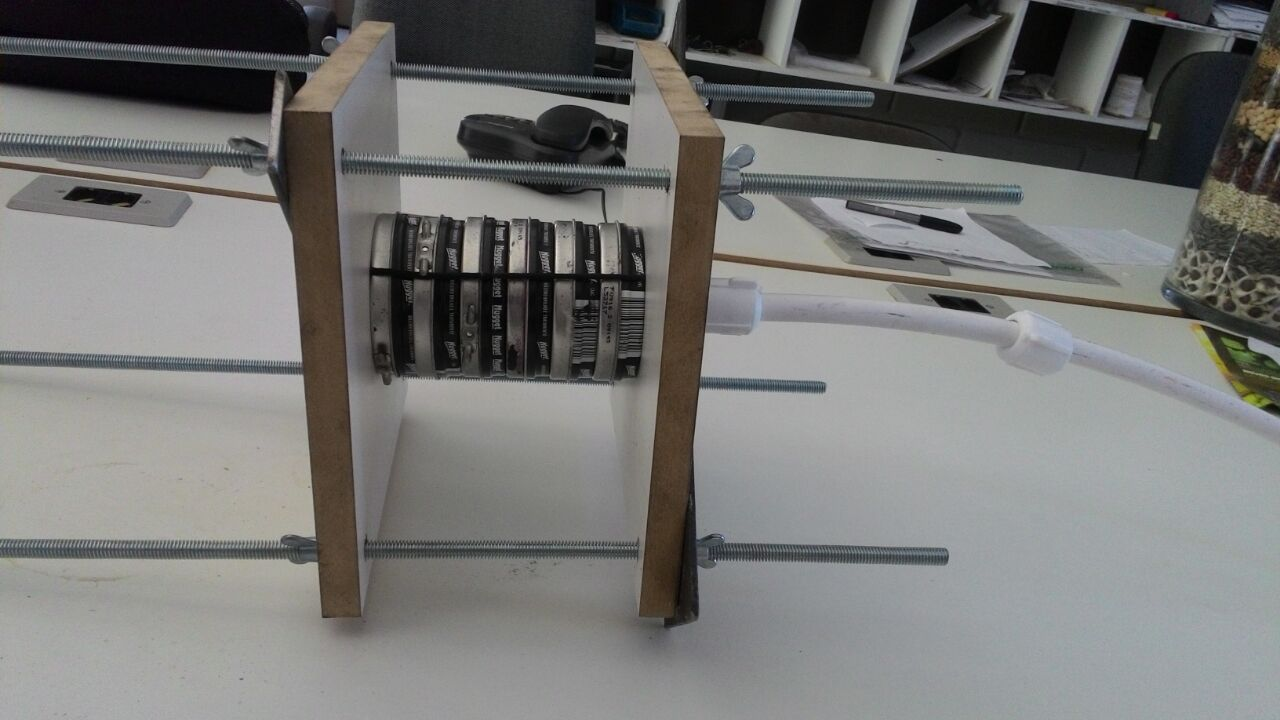
\includegraphics[width=0.9\textwidth]{figuras/segundo_teste.png}
  \caption{Montagem para o segundo teste.\label{fig:segundo_teste}}
\end{figure}


\section{Terceiro teste}\label{sec:terceiro_teste}

Foi trocada a mangueira do primeiro teste por uma de menor diâmetro externo e
com paredes mais finas, possibilitando ser introduzida dentro do adaptador e
alcançando a primeira lata, reduzindo então as possibilidades de vazamento. Para
resolver o problema do teste anterior, a tampa da primeira membrana filtrante
foi colada à placa de madeira e vedada, junto à mangueira com silicone, de modo
a evitar a saída de solução entre a placa e a primeira membrana. Feito o teste,
a solução que entrava suja passou sair mais limpa por as membranas, mas a
pressão de saída da solução na garrafa PET ainda foi um problema. Nesse teste e
nos anteriores, a solução a ser filtrada usada era água com terra.

\begin{figure}[H]
  \centering
  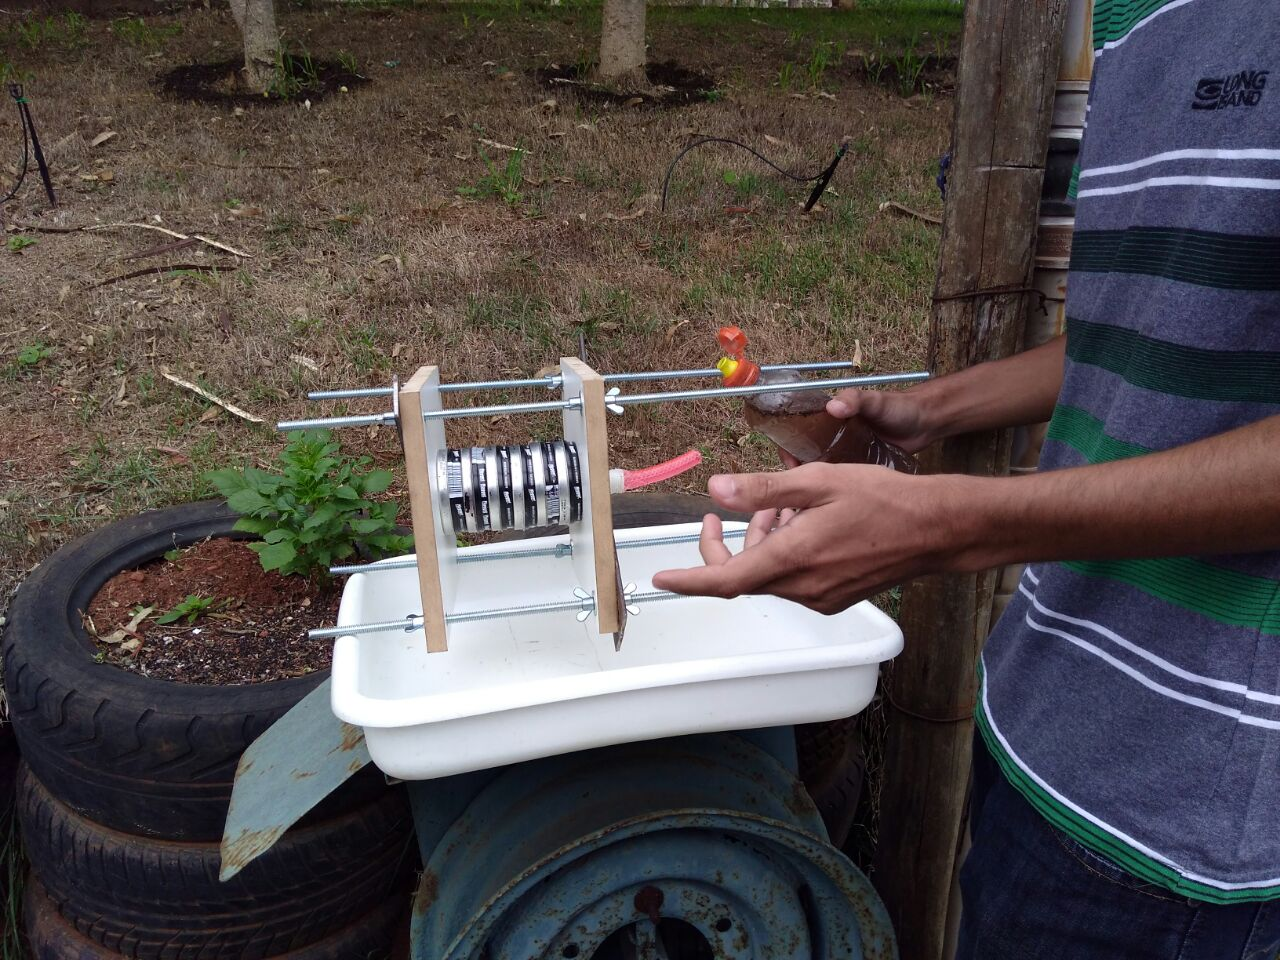
\includegraphics[width=0.9\textwidth]{figuras/terceiro_teste.png}
  \caption{Terceiro teste.\label{fig:terceiro_teste}}
\end{figure}


\section{Quarto teste}\label{sec:quarto_teste}

Para resolver o problema da pressão, o bico da garrafa foi acoplado de forma
fixa à mangueira separadamente e depois conectado a garrafa, tornando o sistema
fechado. Também foi feita uma extensão da mangueira para facilitar o manuseio da
fonte de solução (garrafa contendo a alimentação). Dessa vez, o filtro funcionou
de forma eficiente, o líquido filtrado estava limpo e saindo por todas as
membranas filtrantes. A saída de solução impura pela garrafa PET estava com
pressão satisfatória, devido à boa vedação do sistema. Nesse teste, a solução
usada para ser filtrada foi água misturada com pó de café, fubá, trigo para
quibe e canjiquinha. A escolha dessa solução foi para posterior observação das
partículas retidas pelo algodão.

\begin{figure}[H]
  \centering
  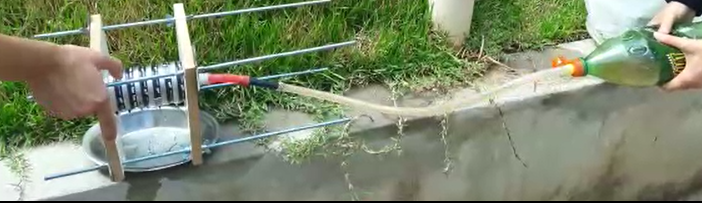
\includegraphics[width=0.9\textwidth]{figuras/quarto_teste.png}
  \caption{Montagem final do quarto teste.\label{fig:quarto_teste}}
\end{figure}


\section{Quinto teste}\label{sec:quinto_teste}

Ainda foi feito um último teste variando a solução. A mistura de água, pó
de café e fubá passou pelo filtro mas não teve filtração tão efetiva quanto
aquela em que havia trigo para quibe e canjiquinha, já que estas são partículas
maiores. Por isso, foi proposto que no teste anterior, as partículas maiores se
uniram na mangueira e formaram um meio filtrante, fazendo com que a solução
entrasse já pré-filtrada no sistema.


%%% Local Variables:
%%% mode: latex
%%% TeX-master: "../main_archive"
%%% End:
